% ---- ETD Document Class and Useful Packages ---- %
\documentclass{ucetd}

\usepackage{subfigure,epsfig,amsfonts}
\usepackage{amsfonts}
\usepackage{natbib}
\usepackage{amsmath}
\usepackage{amssymb}
\usepackage{amsthm}
\usepackage{url}
\usepackage{appendix}

\usepackage{graphicx}
%\usepackage[inkscape={/Applications/Inkscape.app/Contents/Resources/bin/inkscape -z -C}]{svg}
%\usepackage{subfigure}
%\usepackage{subcaption}

%\addbibresource{bibliography.bib}
%\bibliography{bibliography.bib}

% custom commands
\newcommand{\code}[1]{\texttt{#1}}
\newcommand{\eqbegin}{\begin{equation*} \begin{aligned}}
\newcommand{\eqend}{\end{aligned} \end{equation*}}

%% Use these commands to set biographic information for the title page:
%%\title{Effects of a Degraded Network on Hadoop with Erasure Encoded Storage}

\title{Degraded Network Handling by Hadoop with Erasure Encoded Storage}
\author{Joseph A. Ellis}
\department{Computer Science}
\division{Physical Sciences}
\degree{Master of Science}
\date{June 2015}

%% Use these commands to set a dedication and epigraph text
%\dedication{Dedication Text}
%\epigraph{Epigraph Text}


\begin{document}
%% Basic setup commands
% If you don't want a title page comment out the next line and uncomment the line after it:
\maketitle
%\omittitle

% These lines can be commented out to disable the copyright/dedication/epigraph pages
\makecopyright
%\makededication
%\makeepigraph


%% Make the various tables of contents
\tableofcontents
\listoffigures
%\listoftables

%------------------------------------------------------------------------------%

%\acknowledgments
% Enter Acknowledgements here

%------------------------------------------------------------------------------%

\abstract

Erasure encoding storage, a storage technique which encodes parity blocks from
file blocks in order to allow reconstruction of missing or corrupt blocks, is
becoming a popular distributed storage method that reduces storage overhead
while maintaining reliability. In order for erasure codes to perform effectively
as a distributed storage mechanism, node failures and hardware degradation must
be handled appropriately.  Hadoop's current method of handling a degraded
network, known as speculative execution, relies on the fact that replicas of
data exist, but because replicas of data do not exist when using erasure encoded
storage this method must be reevaluated.  Although previous work has studied
both improvements to erasure encoded storage's performance during node failure
and Hadoop's ability to handle a degraded network when using replication,
Hadoop's ability to handle a degraded network when using erasure encoded storage
has yet to be studied.

This paper shows that speculative execution is harmful when using erasure
encoded storage and a cluster's network is degraded and presents speculative
reconstruction, a mechanism to better handle a degraded network in this
situation. By utilizing the fact that erasure encoded storage allows a file
block to be reconstructed, speculative reconstruction is able to avoid waiting
for a block to be transferred over a degraded network link by reconstructing the
block from blocks that can be read over fast network links.

%------------------------------------------------------------------------------%

\mainmatter
% Main body of text follows

%------------------------------------------------------------------------------%

\chapter{Introduction}
\label{ch:introduction}

As data centers continue to grow, the practice of replicating data to ensure
reliability and availability becomes more costly and less practical. For
example, the default replication factor in distributed file systems such as HDFS
is 3, which results in an overhead of 200\% when storing any data. Due to the
high cost of replicating data, erasure encoding storage has begun to gain
popularity and become a method available in several distributed storage systems
\cite{Fan, Calder}. Erasure encoding data allows a storage system to guarantee
the same reliability as replication while reducing the storage overhead to less
than 50\%.

Another problem affecting growing data centers is the increased occurrence of
degraded hardware faults. Many distributed systems are designed to handle
hardware failures but are lacking mechanisms to deal with degraded hardware that
is underperforming \cite{Do}. As compute clusters continue to grow, the
probability of a node suffering from hardware degradation increases, which
means the systems managing these clusters must handle the fault appropriately or
risk suffering severely degraded performance. Because cluster performance can be
seriously reduced by even a single node with degraded network hardware, erasure
encoded storage must be able to efficiently handle a degraded network in order
to provide its storage cost benefits at an acceptable level of performance.

In this study, I investigate the current state of Hadoop with erasure encoded
storage and its ability to handle a degraded network. I show that the use of
speculative execution is not the proper mechanism for handling a degraded
network, due to its reliance on the availability of data replicas. Because
speculative execution does not effectively handle a degraded network when data
is erasure encoded, I propose speculative reconstruction.  Speculative
reconstruction takes advantage of erasure encoded storage's ability to
reconstruct data blocks and utilizes the cluster's fast network links to do so,
which allows data to be retrieved from HDFS without waiting for data transfers
over the slow network link.

%------------------------------------------------------------------------------%

\chapter{Background}
\label{ch:backgroud}

In this work, I will be using the Hadoop Distributed File System (HDFS) and the
Hadoop MapReduce framework in order to understand how an erasure encoded storage
system handles a degraded network. HDFS currently uses replication and
stores massive data sets on the order of petabytes or greater, which provides an
ideal situation to optimize data storage techniques in order to reduce the
cost of providing reliable data storage. Hadoop \cite{Hadoop} is currently able to
provide erasure encoded storage through a separate module known as HDFS-RAID
\cite{HDFS-Raid}, although it will soon provide full support for erasure encoded
storage \cite{HDFS-EC:Design}.

\begin{figure}
    \centering
    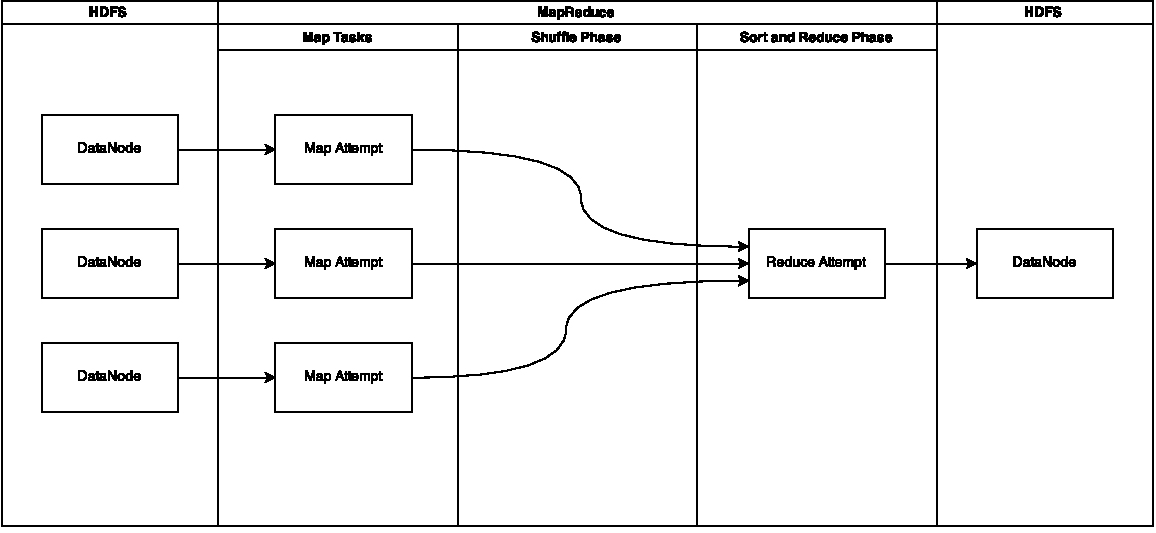
\includegraphics[width=\linewidth]{diagrams/HadoopJobCrossSection.pdf}
    \caption[Hadoop Job Cross Section]{Cross section of a Hadoop job
        showing the flow of data.}
    \label{crossSect}
\end{figure}


\section{HDFS}

The Hadoop Distributed File System is one of the most widely used distributed
file systems due to the fact that it is able to provide data reliability and
availability guarantees while running on commodity hardware that is expected to
experience failures \cite{HDFS-Arch}. Like other file systems, HDFS stores files
as a series of blocks, although HDFS blocks are much larger (64 MB by default)
in order to reduce seek time when reading large files. A key difference between
HDFS and standard file systems is that it ensures data reliability and
availability.  In order to do this HDFS replicates each data block and
distributes blocks across multiple nodes.  By default, HDFS replicates each
block 3 times and places each replica on a separate datanode to ensure it can
recover from up to 2 node failures. By replicating each data block across
multiple nodes, HDFS is able to recover from block loss or corruption by reading
the data block from one of the replicas.

\section{Hadoop MapReduce}

Hadoop's MapReduce framework is also widely used and integrated with HDFS. The
MapReduce framework allows computations to be distributed and run over the large
data sets stored in HDFS.  It operates by partitioning a computation into tasks
and then distributing the tasks across the cluster to be run on individual sets
of data blocks. The two main components of a MapReduce job are the map tasks and
reduce tasks, while speculative execution is the current method for handling
cases when these tasks appear to be running slowly. Hadoop defines a job as the
entire computation over a data set, a task as a computation on some subset of
input or intermediate data, and an attempt as a specific instance of task
execution.

    \subsection{Map Task}

The map task is a computation defined as a function of some input key/value pair
with type $\langle \tau_1 \times \tau_2 \rangle$ that outputs zero or more
intermediate key/value pairs with type $\langle \tau_1^{\prime} \times
\tau_2^{\prime} \rangle$. The MapReduce framework then provides the individual
map tasks with a subset of the input data, the size of which is determined by
the Hadoop file format used to store the data. Once the map task has completed,
the intermediate pairs it produces are used as input to the reduce phase.

    \subsection{Reduce Task}

A reduce task is the secondary computation run that ``reduces a set of
intermediate values which share a key to a smaller set of values.''
\cite{Reducer} The input to reduce tasks is the intermediate key/value pairs
produced by mappers grouped by key and has type $\langle \tau_1^{\prime} \times
List(\tau_2^{\prime}) \rangle$ where $List(\tau_2^{\prime})$ is the list of all
values sharing the same key.  The reduce task is broken up into three phases:
shuffle, sort, and reduce.  During the shuffle phase, the reduce task copies its
partition (as defined by the \code{Partitioner}) of the intermediate Key/Values
from every mapper. The sort phase runs at the same time as the shuffle phase and
sorts each copied input by key. Once all of the inputs are sorted, the reduce
phase runs and reduces each each input pair to some final output, which is
usually written to HDFS.

    \subsection{Speculative Execution}

An important feature of the MapReduce framework is speculative execution, which
is a mechanism designed to reduce the overall runtime of jobs by executing a
backup attempt for a specific task when that task appears to be running slowly.
The general idea is that a task is running slowly due to the resources it is
using, so a backup task can be completed more quickly by using a different set
of resources.  Figure \ref{specExec} shows a map task that must read block B
where the initial map attempt is assigned to read from DataNode 1 which has a
degraded network connection, running at only 1Mb/s. Speculatively executing a
backup map attempt results in a replica of block B being read from DataNode 2
with a properly functioning network connection, allowing the backup attempt to
finish before the original map attempt. Although
not always the case \cite{Do}, speculative execution has proven to be a
successful method of handling many faults and improving performance when data is
replicated across several nodes \cite{Dean:SpecExec}.

\begin{figure}
    \centering
    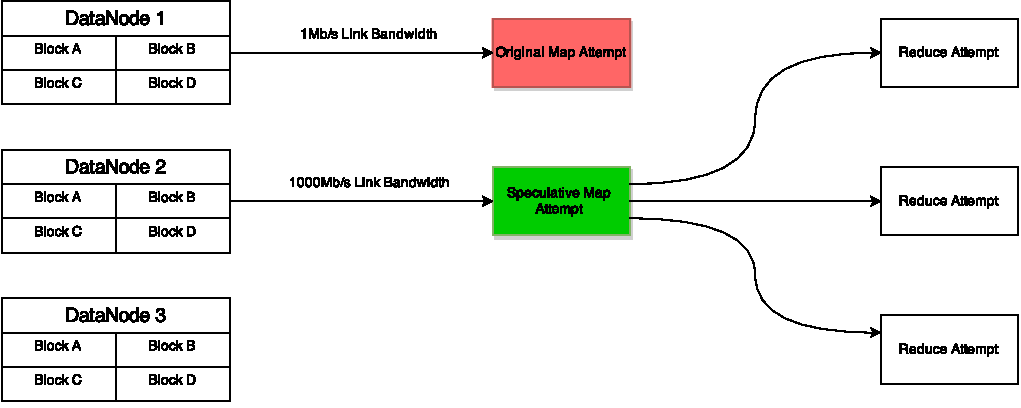
\includegraphics[width=\textwidth]{diagrams/SpeculativeExecution.pdf}
    \caption{Speculative Execution}
    \label{specExec}
\end{figure}

\section{Erasure Codes}

Erasure codes provide a way to encode redundant data as a function of the input
data such that the original data is able to be recovered when data loss or
corruption occurs. With regard to HDFS this means that parity blocks are encoded
from file blocks and the set of file and parity blocks provide a means to
recover the original data file when some subset of these blocks are lost for any
reason.  Reed-Solomon codes are of great interest because the storage overhead
required to store the encoded parity blocks is relatively low.

    \subsection{Reed-Solomon Codes}

Reed-Solomon codes have been commonly used to correct for errors in data storage
and have also been used in conjunction with HDFS. Reed-Solomon codes allow $M$
data blocks to be encoded into $K$ parity blocks, where $K$ is the number of
missing or corrupted blocks (erasures) that can occur while still allowing the
original data to be recovered \cite{Reed}. The literature uses the notation
$RS(M,K)$ when referring to Reed-Solomon codes with specific values for $M$ and
$K$.  This scheme conveniently allows a user of the codes to examine the trade
off between reliability needs and storage costs for their specific use case and
modify the number of parity blocks to be computed and stored.

    \subsection{HDFS-Raid}

HDFS-Raid \cite{HDFS-Raid} is currently the system that allows HDFS to provide
erasure encoded storage through the use of the Reed-Solomon codes. HDFS-Raid is
designed such that a separate process, called the \code{RaidNode}, handles the
initial encoding of data along with repairing any corrupt or missing blocks. Any
reads to corrupt or missing blocks are recomputed on the fly by mappers using
the \code{DistributedRaidFileSystem}.  This allows HDFS to continue to provide
data to the application even when faced with missing or corrupt data blocks.

When using Reed-Solomon codes with HDFS, the value of $M$ is known as the
stripe length and the value of $K$ is known as the parity length. The stripe
length is equal to the number of file blocks that should be encoded into $K$
parity blocks, allowing the file to recover from up to $K$ blocks of original or
parity data to be lost or corrupted. A concrete example is $RS(5,2)$, which
allows a stripe's data to be retrieved when up to 2 blocks are corrupt or missing.

An important difference between erasure codes and replication is the block
placement policy. When blocks are replicated, as long as each block replica is
placed on a different node, HDFS is able to withstand $N - 1$ node failures,
where $N$ is the number of block replicas. When using erasure codes, each
stripe's data blocks and parity blocks are unique and must be placed on
different nodes, a policy known as striping. If two blocks that are part of the
same stripe are collocated, a single node failure can cause multiple blocks to
be lost which reduces the number of failures a file is able to withstand and
effectively negates the benefits of using erasure codes. Figure \ref{striping}
shows how striping places data and parity blocks on distinct datanodes when one
file consists of blocks A and B, another file consists of blocks Y and Z, and
the parity blocks AB and YZ encode their respective file blocks.

\begin{figure}[h]
    \centering
    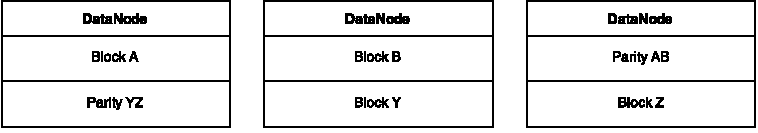
\includegraphics[width=\textwidth]{diagrams/Striping.pdf}
    \caption{Striping}
    \label{striping}
\end{figure}

%------------------------------------------------------------------------------%

\chapter{Related Work}

Previous work has studied Hadoop's performance while a cluster suffers from
degraded hardware along with performance improvements to erasure encoded
storage. It has been shown that distributed systems are able to reduce the
latency of the slowest jobs by issuing requests to multiple replicas of a
resource and accepting the response of the fastest request. Work has also shown
degraded hardware is a serious problem and that even a single node with degraded
hardware is able to severely hinder cluster performance. New erasure codes have
been designed for use specifically with distributed erasure encoded system,
which reduce the disk and network I/O required during the reconstruction
process. Scheduling tasks that require block reconstruction first has been shown
to reduce resource competition and job runtime. Finally, distributed storage
systems have been designed that utilize erasure codes while reducing the latency
of read and write operations.

\section{Latency Tail}

As distributed systems continue to grow, the variability of response times
continues to increase as a result of many factors including shared resources and
maintenance activities \cite{Dean:Tail}. This increase in variability results in an
increase in the fraction of jobs that take longer than a given time to complete,
known as high tail latency. One method of handling this variability in a
distributed system is, ``to issue the same request to multiple replicas and use
the results from whichever replica responds first'' \cite{Dean:Tail}. Hadoop's
speculative execution mechanism is designed as a variation of this idea by
executing backup attempts for tasks that appear to be running slowly. The
problem with trying to reduce tail latency in this manner when using erasure
encoded storage is that there are not multiple replicas. Instead a new method of
tail latency reduction must be designed for systems that do not have the
option to issue the same requests to multiple replicas.

\section{Degraded Hardware}

There have been some studies on the effects of degraded hardware on cloud
systems that show how serious these types of faults can be. Do et al. \cite{Do}
find that one node with degraded hardware can bring the entire system
down, even for a system that is designed to handle such faults. Their work
motivates research into how new types of failures, such as degraded hardware,
affect systems and how these failures might be remedied in system design and
implementation. My research builds on their ideas by looking at a specific
system implementation, finding a weakness to degraded resources, and offering a
solution that helps reduce the effect of such a failure.

\section{New Erasure Codes}

While erasure codes provide the means to recover corrupt or lost data, the cost
of reconstructing the lost data comes in the form of increased disk and network
utilization. In order to reduce these costs, new types of erasure codes, known
as Local Reconstruction Codes (LRC), that are designed to take advantage of data
locality have been designed and analyzed for use in distributed storage systems
such as Windows Azure \cite{Huang} and HDFS \cite{Sathiamoorthy}. These codes
attempt to provide similar performance, in terms of time, when compared to
currently used codes like Reed-Solomon, while reducing the disk and network
costs of block reconstruction. Xorbas is an example of a system that implements
LRC for use with HDFS and is able to provide a reduction in disk I/O and network
traffic by 2x at a storage cost of 14\%  \cite{Sathiamoorthy}. By reducing disk
and network usage, these LRCs may be able to reduce the effects of degraded
networks during the reconstruction process, but do not affect the performance of
jobs when a system is suffering from a degraded network because the
reconstruction process is never invoked.

\section{Job Scheduling}

Other aspects of how to handle failures when using erasure encoded storage have
been investigated, specifically how to schedule degraded read tasks (tasks that
must recompute their data block) \cite{Li}. Scheduling these tasks first appears
to improve overall performance by reducing competition for resources. This
scheduling only comes into effect when a data block is missing or corrupted and
not when a node is suffering from degraded hardware, so it doesn't solve the
problem of a degraded network, which isn't considered a failure. Although it
doesn't solve this specific problem, Degraded-First Scheduling does appear to
complement speculative reconstruction by reducing resource competition when
reconstruction tasks are executed.

\section{Distributed Storage}

RobuSTore \cite{Xia} is an example of a distributed storage system that is
designed to utilize the fact that erasure codes allow a unique means to access
stored data. By storing a number of encoded blocks across multiple servers, a
read request is able to be probabilistically satisfied by the fastest storage
servers by requesting all of the file's blocks and cancelling the slow requests
once a sufficient set of blocks have been received such that the data can be
decoded.  They show this method provides higher bandwidth, when utilizing many
disks and servers, along with lower latency variance since the request only
needs a subset of the total file blocks, which can likely be read from fast
servers. This systems seems to work well when the entire file is being
requested, however the MapReduce framework operates differently in that the
computation is distributed and each mapper only needs a portion of the input
file.  RobuSTore would likely perform poorly in this setting because in order
for each mapper to retrieve its subset of the input file it would need to
acquire enough file blocks to recover the entire file, introducing a huge
overhead compared to that of reading a single decoded block.  In order for a
system like this to work, there needs to be more fine grained control over how
files are able to be read, specifically how to efficiently retrieve file blocks,
as is required by MapReduce.

\section{Discussion}

While these works have provided solutions, improvements, and insights into the
handling of degraded hardware and the performance of Hadoop and erasure encoded
storage, they have not provided a mechanism or system that allows Hadoop to
effectively handle a degraded network when using erasure encoded storage. My
work shows that Hadoop with erasure encoded storage does not gracefully handle
a degraded network and proposes a new degraded network handling mechanism to
supplement the previous work done to improve performance and reduce latency of
distributed erasure encoded storage systems.

%------------------------------------------------------------------------------%

\chapter{Experiments and Results}

\section{Setup}

The experiments were run using Hadoop 0.23.11 \cite{Hadoop:0.23.11} for both HDFS and MapReduce along
with HDFS-Raid 0.22.0 \cite{HDFS-Raid}. These were setup on an Emulab \cite{Emulab} cluster with
9 nodes: 1 node acting as the manager, 4 as NodeManagers, and 4 as DataNodes.
The reason for running the NodeManagers and DataNodes on separate machines is to
ensure that reading data from a DataNode is the only operation that occurs over
the degraded network connection along with ensuring that no map or reduce tasks
are executed on the node with the degraded network connection. All tests were
run on Emulab pc3000 machines, which are Dell PowerEdge 2850s with a single 3GHz
processor, 2GB of RAM, and 2 10,000 RPM 146GB SCSI disks. Each node was
configured to have one of the 146GB disks mounted as storage for HDFS. HDFS was
configured to use the default block size of 64MB.

\section{Test Methods}

HDFS-Raid was run with (5,2) Reed-Solomon enabled and a 5 block ($\sim$300MB)
file was generated that was erasure encoded with 2 parity blocks. The MapReduce
job used is a modified version of a SWIM job \cite{SWIM}. A SWIM job is a
MapReduce job defined by \code{WorkGen.java} and consists of a mapper and
reducer, each of which produce a modifiable ratio of output pairs to input
pairs. Because I am only interested in the read performance of HDFS, the ratio
used for both the map and reduce tasks is 0. This means that the job simply
reads each input Key/Value pair from the file and does nothing with it.

The \code{FileFormat} used by the SWIM job is the \code{SequenceFileFormat}.
This format splits the job input based on block size so that the number of maps
is equal to the number of blocks in the file. Because of this splitting
technique, one map task will be assigned to the block located on the node with a
degraded network making the effect of the degraded network obvious in the
performance of that task.

Simulating a degraded network was done by using Emulab's own network simulation
software. This software allows the bandwidth of a given node's network
connection to be dynamically modified. This allowed for network links with
bandwidths from 10Mb/s to 1Mb/s to be simulated.

After the input was generated using the \code{HDFSWrite} class included with
SWIM, one of the four datanodes containing only one data block had its network
connection set to the desired bandwidth. The job was then run and the job, task,
and attempt data were recorded by Hadoop and collected using the
\code{HistoryServer} Rest API.

\section{Results}

Hadoop's HistoryServer collects many statistics about an individual job's
execution so all necessary data was collected using a Python script that scraped
data using the HistoryServer's Rest API. The most relevant statistic recorded
was the start and end time of each attempt which was plotted using swimlane
plots \cite{Tan}. These plots show the individual runtimes of each attempt,
relative start and end times, and any backup attempts that were executed for
each task. 

After collecting and plotting the data, the runtime of each individual task
attempt that the MapReduce framework made was analyzed. In the swimlane plots
(Figures \ref{fig:10Mb}, \ref{fig:5Mb}, \ref{fig:2-5Mb}, \ref{fig:1Mb})
for jobs that were run without speculative execution, we can clearly see one map
attempt that takes far longer than the others indicating that it is the one
reading over the slow network. This behavior meets expectations since a map task
that is assigned to read from a slow datanode will not fail but rather wait for
the read operation to complete regardless of the rate.

The swimlane plots depicting the jobs that were run with speculative execution
enabled show much worse performance than their non speculative counterparts. We
see that when a backup attempt is executed in an effort to speed up the slow map
task, the task actually takes longer to complete. Because the file was erasure
encoded, the original attempt and secondary attempt are forced to read from the
same datanode and thus share the datanode's slow network connection, as shown in
Figure \ref{specExecEras}. In this case, the original map attempt still tends to
finish first, since it has already partially completed its read before the
backup attempt starts, but sharing the slow link causes the task to take twice
as long to complete relative to the same job run without any speculative
execution.

\begin{figure}
    {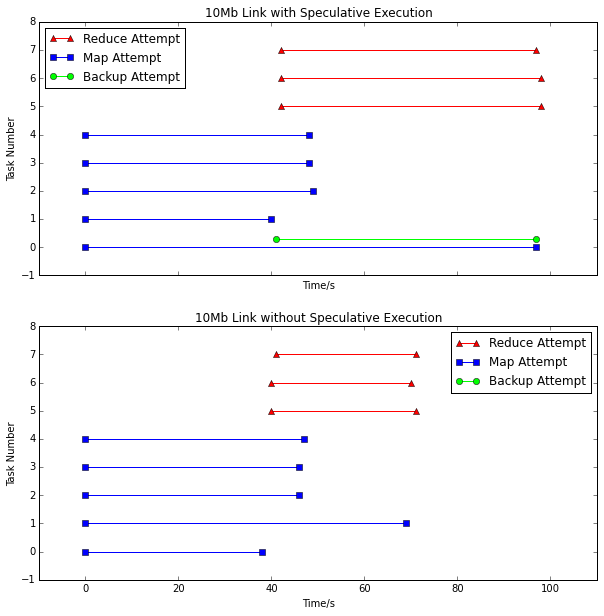
\includegraphics[width=\textwidth]{plots/10Mb.png}}
    \caption[Tests with link bandwidth of 10Mb/s]{SWIM job run with one node's
    bandwidth set to 10Mb/s}
    \label{fig:10Mb}
\end{figure}

\begin{figure}
    {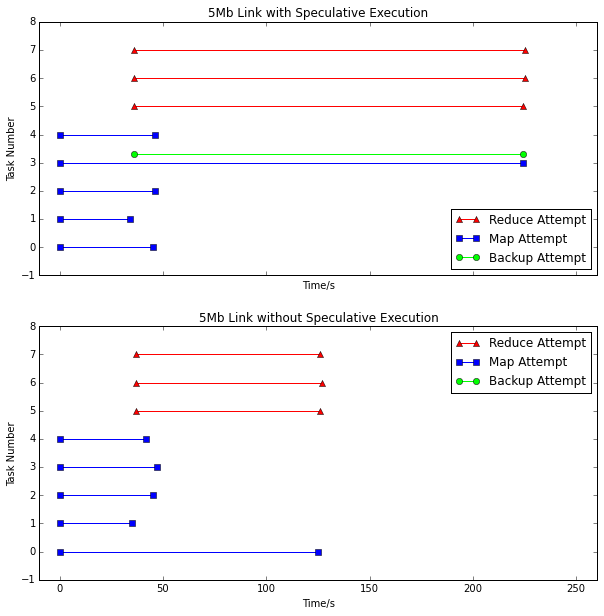
\includegraphics[width=\textwidth]{plots/5Mb.png}}
    \caption[Tests with link bandwidth of 5Mb/s]{SWIM job run with one node's
    bandwidth set to 5Mb/s}
    \label{fig:5Mb}
\end{figure}

\begin{figure}
    {\includegraphics[width=\textwidth]{plots/2-5Mb.png}}
    \caption[Tests with link bandwidth of 2.5Mb/s]{SWIM job run with one node's
    bandwidth set to 2.5Mb/s}
    \label{fig:2-5Mb}
\end{figure}

\begin{figure}
    {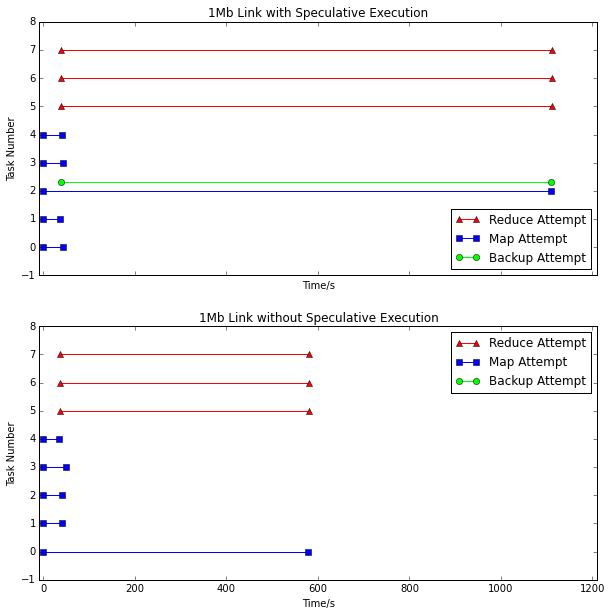
\includegraphics[width=\textwidth]{plots/1Mb.png}}
    \caption[Tests with link bandwidth of 1Mb/s]{SWIM job run with one node's
    bandwidth set to 1Mb/s}
    \label{fig:1Mb}
\end{figure}

\begin{figure}
    \centering
    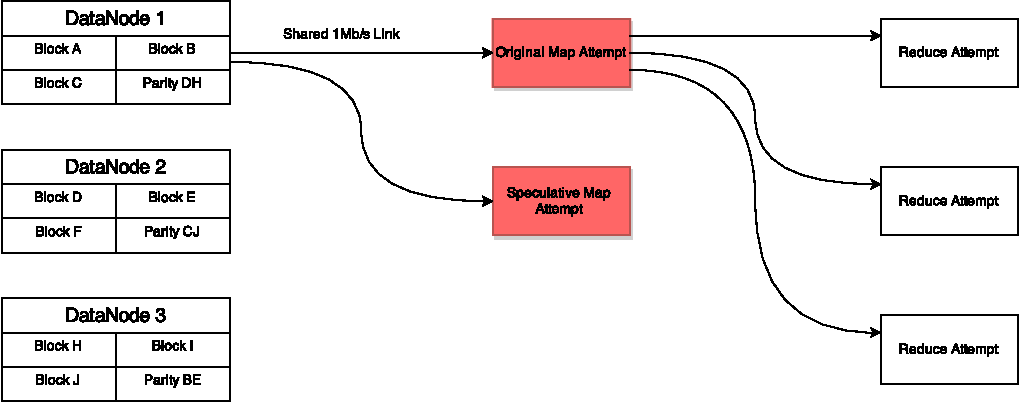
\includegraphics[width=\textwidth]{diagrams/SpeculativeExecutionErasureCodes.pdf}
    \caption[Speculative Execution and Erasure Codes]{Speculative execution when
    data is erasure encoded causes the slow link to be shared, which results in
    further performance degradation.}
    \label{specExecEras}
\end{figure}

%------------------------------------------------------------------------------%

\chapter{Speculative Reconstruction}

I have shown that speculative execution does not work as intended when data
is erasure encoded because the speculative attempt competes with the original
attempt for network resources over an already degraded connection. This not only
means that speculative execution should not be used when data is erasure
encoded, but also that a new mechanism must be designed if erasure encoded
storage is going to be able to perform acceptably when a degraded network
occurs. Speculative reconstruction is a mechanism designed to handle degraded
networks in an effective manner when using erasure encoded storage.

The idea behind speculative reconstruction is that at some point it becomes
faster to read the rest of data stripe and reconstruct a data block than it is
to read a block over a slow network connection.  Speculative reconstruction is
similar to speculative execution in that a backup task is executed in an attempt
to reduce the overall runtime of the job, although instead of attempting to read
the same data block, the backup task recomputes the data block using the rest of
the stripe's blocks.  As a method of fault recovery, speculative reconstruction
does not rely on the assumption that there are multiple replicas of each data
block, but rather on the ability to retrieve a block's data without ever
interacting with the node that the block is stored on.

When a datanode's network link is degraded and data is erasure encoded, a map
task with its input stored on that datanode is forced to read the block over the
degraded connection. Figure \ref{specRecon} illustrates this scenario and shows
the first map task attempting to read block B over a degraded network
connection. Once the original map attempt is determined to be running slowly,
the speculative attempt can be executed and begin reading the data blocks in
block B's stripe, block E and parity block BE in this case. Because the rest of
the stripe's blocks are stored on nodes with properly functioning network
connections, the speculative attempt is able to quickly retrieve the stripe's
blocks, reconstruct block B, and complete the map task without ever accessing
block B or using the degraded network connection.

\begin{figure}
    \centering
    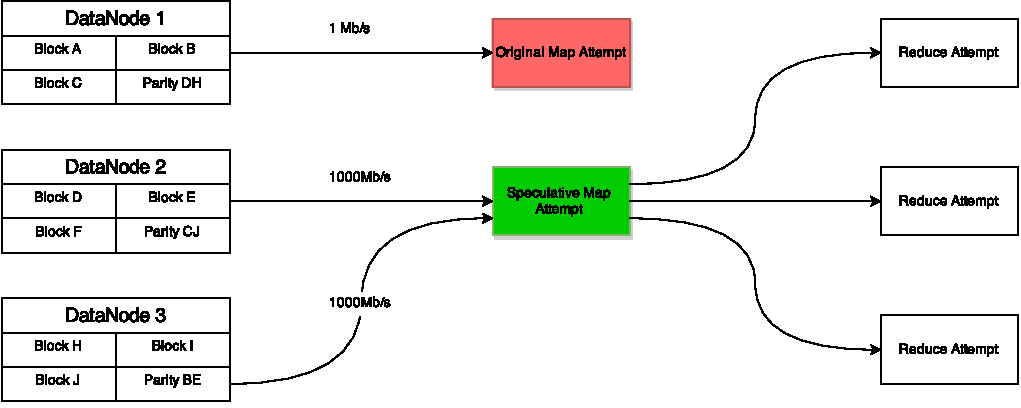
\includegraphics[width=\textwidth]{diagrams/SpeculativeReconstruction.pdf}
    \caption[Speculative Reconstruction]{A speculative reconstruction attempt
        reads the remaining file blocks and parity blocks and reconstructs the
        original data block for processing.}
    \label{specRecon}
\end{figure}

\section{Analytical Model}

In order to show that speculative reconstruction is a viable method of handling
a degraded network, I first develop an analytical model that compares the cost
of block reconstruction with the cost of retrieving a block over a degraded
connection.  This model is intentionally general and assumes things like
constant and known network bandwidths. These assumption are made because the
purpose of this model is not to compute exact values for the cost of
reconstruction or slow reads, but to estimate the severity of network degradation
that must occur in order for speculative reconstruction to be considered as an
effective alternative to reading the block. The following definitions will be
used when defining the model:

\begin{description}
    \item[Block Size]% \hfill \\
        size of a block in HDFS
    \item[Reconstruct Time]% \hfill \\
        time required to reconstruct a block from $M$ other blocks in its stripe
    \item[Expected Bandwidth]% \hfill \\
        minimum available bandwidth between the compute node and any datanode
        storing a block in the stripe excluding the original block
    \item[Slow Bandwidth]% \hfill \\
        available bandwidth between the compute node and the datanode storing
        the original block
\end{description}

For speculative reconstruction to perform better than reading over a slow network
connection, the cost of reading $M$ other blocks plus the cost of reconstruction
must be less than the cost of reading the block over the slow connection:
\eqbegin
    M \times \frac{\text{block size}}{\text{expected bandwidth}} + \text{recompute time}
    < \frac{\text{block size}}{\text{slow bandwidth}}
\eqend
but since each of the blocks are able to be read in parallel we have:
\eqbegin
    \frac{\text{block size}}{\text{expected bandwidth}} + \text{recompute time}
    < \frac{\text{block size}}{\text{slow bandwidth}}
\eqend
If we define $R$ as the ratio of expected bandwidth to slow bandwidth such that:
\eqbegin
\text{expected bandwidth} = R \times \text{slow bandwidth}
\eqend
we can define the relationship between reconstruction time and time taken to
read a slow block:
\eqbegin
    \frac{\text{block size}}{\text{expected bandwidth}} + \text{reconstruct time}
    &< \frac{\text{block size}}{\text{slow bandwidth}} \\
    \text{reconstruct time}
    &< \frac{\text{block size}}{\text{slow bandwidth}} - \frac{
        \text{block size}}{R \times \text{slow bandwidth}} \\
    \text{reconstruct time}
    &< \frac{(R - 1) \times \text{block size}}{R \times \text{slow bandwidth}} \\
    \text{reconstruct time}
    &< \frac{R - 1}{R} \times \text{slow block read time} \\
\eqend
where `slow block read time' is equal to $\frac{\text{block size}}{\text{slow
bandwidth}}$. Reconstruct time is left as an imprecise value because the actual
time taken to reconstruct a block depends greatly on the erasure code
implementation and hardware being used. This model gives us a simple way to
determine how degraded a network connection must be relative to the rest of the
cluster's network in order for block reconstruction to outperform the block
read.

It is worth mentioning that this model can be made more general by defining it
in terms of block retrieval time rather than in terms of network bandwidths. We
can redefine $R$ such that:
\eqbegin
    \text{expected retrieval time} = R \times \text{slow retrieval time}
\eqend
where retrieval times represent the time taken for a compute node to access a
data block. The general form of the model then becomes:
\eqbegin
    \text{reconstruct time}
    &< \frac{R - 1}{R} \times \text{slow retrieval time} \\
\eqend
This redefinition then allows the model to be applied when determining if
reconstruction is effective not only when analyzing degraded networks, but also
things such as degraded disks or resource competition that results in slow
retrieval times.

\section{Preliminary Tests}

Speculative execution is not currently implemented, so in an attempt to see what
type of performance can be expected when reconstructing a data block, the same
test described previously was run, except rather than slowing the bandwidth of a
particular node the datanode process of a node was killed. Killing the datanode
process simulates a missing block and triggers the reconstruction process. By
triggering the reconstruction process we are able to get an idea of the cost of
block reconstruction. The test was run with both $RS(5,2)$, as in the previous
tests, along with $RS(6,3)$ where 9 nodes were set up to run as both
nodemanagers and datanodes.

\begin{figure}
    {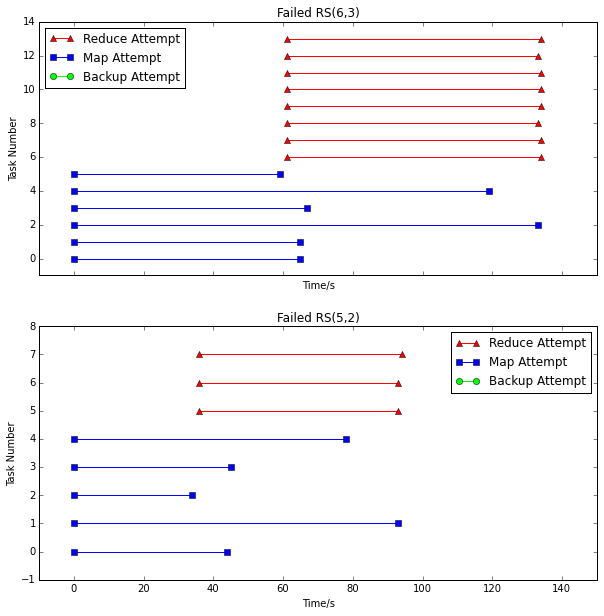
\includegraphics[width=\textwidth]{plots/recompute.png}}
    \caption[Block Reconstruction Tests]{SWIM job run with one killed datanode
    process forcing block reconstruction.}
    \label{recompute}
\end{figure}




\section{Results}

\subsection{Redundant Reconstruction}

\begin{figure}
    \centering
    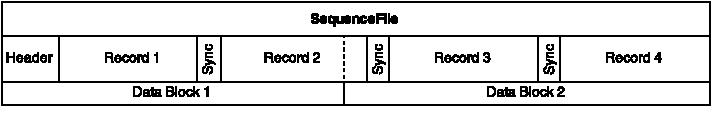
\includegraphics[width=\textwidth]{diagrams/SequenceFile.pdf}
    \caption[Sequence File Format]{The Sequence File Format with one record
        overlapping the boundary between two data blocks.}
    \label{seqFile}
\end{figure}

The most notable artifact seen in the swimlane plot (Figure \ref{recompute}) is
that two of the map tasks took longer to complete in each job, indicating that
they were both forced to recompute a block. This is interesting because only one
block was not accessible and each map task's input is an individual block. The
reason this occurred is because the \code{SequenceFileFormat} is used to store
the input file in HDFS and it stores records which are not necessarily aligned
with the block boundaries that HDFS recognizes.  This means that the input block
a mapper is assigned may not contain the entire last record, resulting in the
mapper having to read the remainder of the record from another block.

An example of the boundary mismatch between records and blocks is shown in
Figure \ref{seqFile}, where record 2 overlaps two data blocks. In
this scenario, if data block 2 is missing or corrupt, not only does the mapper
with block 2 as input have to reconstruct the block but the mapper with block 1
as input must also recompute block 2 in order to read the remainder of record 2,
which explains the 2 long running map tasks. The second slow map task is not
seen in the tests with a degraded network because the mapper reads the little
bit of data remaining in the final record over the slow link, which takes a
relatively insignificant amount of time due to the small amount of data being
read.

The fact that a single data block may contain input to more than one map task is
important to consider when deciding how to handle a degraded network because
simply executing speculative reconstruction tasks can result in the same block
being unnecessarily reconstructed multiple times by tasks that are part of the
same job.  In order for speculative reconstruction to be a viable mechanism for
handling degraded networks it must avoid redundant reconstruction which wastes
time and cluster resources.

\subsection{Reconstruction Performance}

Even though one of the mappers was forced to recompute a block from which it
only needed part of one record, the overall runtime of the jobs for both
$RS(5,2)$ and $RS(6,3)$ were significantly faster than previous jobs that had to
read a block over a degraded network connection.  The reconstruction time
appears to take about 45 seconds for $RS(5,2)$ with the cluster set up such that
the 4 datanodes ran separately from the 4 nodemanagers.  When $RS(6,3)$ was used
and 9 nodes running as both datanodes and nodemanagers, which is the standard
way to setup a Hadoop cluster, reconstruction time took around 60 seconds. These
reconstruction times are very promising and show that when using erasure encoded
storage any data block can be retrieved at least as quickly as the time required
to retrieve any $M$ blocks from the same stripe plus the potentially small
amount of time taken to reconstruct the block.

Having collected values for block reconstruct time, the model previously
discussed can be applied in order to determine the factor $R$ by which a
degraded network link must be under performing such that a job can benefit from
speculative reconstruction. 1.6MB/s is used as the expected link
bandwidth because the average read time of a 64MB block is 40 seconds when using
$RS(5,2)$. This is significantly lower than the full network bandwidth of
1000Mb/s, although the reasons for the low bandwidth utilization are not
important for this analysis.

\eqbegin
    45s &< \frac{(R - 1) 64Mb}{R \times \text{slow link bandwidth}} \\
    45s \times \text{expected link bandwidth}
    &< R \times 64 MB - 64MB \\
    45s \times 1.6 MB/s
    &< R \times 64 MB - 64MB \\
    2.125 &< R
\eqend

This shows that it may be beneficial to speculatively reconstruct the block when
the expected network bandwidth is 2.125x greater than a degraded network link,
or when the slow network link has a bandwidth of 0.75 MB/s (6 Mb/s). Figure
\ref{compare} compares the previous tests with the reconstruction test and shows
that this result is supported by the 5Mb/s link test which took 125 seconds to
execute while the reconstruction test only took 100 seconds. These two times
aren't as close as expected, but that's likely because although the datanode in
the test had a 5Mb/s link, it did not have sole control of that link and other
network communications further reduced the available bandwidth resulting in an
increased job runtime.

\begin{figure}[h]
    \centering
    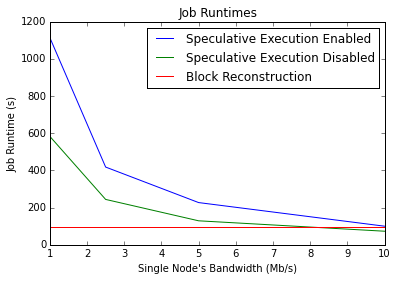
\includegraphics[scale=0.7]{plots/spec_vs_recon.png}
    \caption{Speculative, Nonspeculative, and Reconstruct Job Runtimes}
    \label{compare}
\end{figure}



\section{Drawbacks}

As with speculative execution, determining when speculative reconstruction is
the right choice depends on many factors that are constantly changing. The model
used to compare the cost of reconstruction and the cost of block reads gives
only a general idea of when reconstruction is a viable option and doesn't
consider variations in network bandwidth or block reconstruction time that result
from the many jobs running on the cluster. In practice, it is likely that
determining accurate network bandwidths is too difficult and that the best way
to determine when to speculatively reconstruct a block is similar to
speculative execution's current method, which executes a backup attempt when a
map task is running significantly slower than the job's other maps tasks.

The discussion thus far has also ignored the cost of block reconstruction in
terms of cluster resources.  Speculative reconstruction presents a trade off
between block retrieval time and disk, network, and compute resources.  This
trade off must be carefully analyzed in order to prevent wasteful use of
resources and to prevent further performance degradation through over
utilization of cluster resources.

%------------------------------------------------------------------------------%

\chapter{Future Work}

Although speculative reconstruction appears to be a viable option for dealing
with a degraded network when using erasure encoded storage, it has not yet been
implemented. Implementing and testing speculative reconstruction must be done in
order to verify that it does indeed perform as expected. Once verified, there
are other faults that can occur which speculative reconstruction may or may not
be able to handle. A common occurrence in clusters running on commodity hardware
is degraded disks that begin to underperform in a manner similar to that of the
networks studied here. Speculative reconstruction may provide the answer to
dealing with degraded disks as well, although this has yet to be shown. Another
situation is competition for cluster resources when many jobs run
simultaneously. In scenarios when this competition results in slow block
retrieval, speculative reconstruction may again provide a boost in performance
although this may not always be the case. The large amount of network, disk, and
compute resources required to reconstruct a block may result in speculative
reconstruction further degrading performance. The trade off between resource
utilization and job latency must be analyzed further in order to determine the
scenarios in which speculative reconstruction is the best option and when the
cost of resources is too great to provide a benefit.

%------------------------------------------------------------------------------%

\chapter{Conclusion}

The test results show that speculative execution is not the correct solution to
handling a degraded network when using erasure encoded HDFS. By executing backup
attempts, the degraded network connection becomes more saturated resulting in an
even greater job runtime than if the backup attempt had not been executed. The
detrimental performance of speculative execution in this scenario requires that
a new mechanism be designed to handle a degraded network when using erasure
encoded storage.

Understanding the properties of an erasure encoded storage system allows us to
make new assumptions and design new mechanisms that better handle all types of
faults in the system, included degraded network connections. Speculative
execution utilizes the fact that erasure encoded storage allows the data stored
in a data block to be retrieved through block reconstruction and allows erasure
encoded storage to gracefully handle a degraded network.  By continuing to
develop these types of mechanisms, distributed erasure encoded storage systems
continue to become a more viable solution to reliably storing data at a fraction
of the cost of replication.

%------------------------------------------------------------------------------%

\begin{appendices}
    \chapter{Problems}

    The following describes some of the problems experienced when testing using
    Hadoop, HDFS-Raid, and the SWIM workload.

    \section{Problems with SWIM workload}

    \begin{figure}[h]
        \centering
        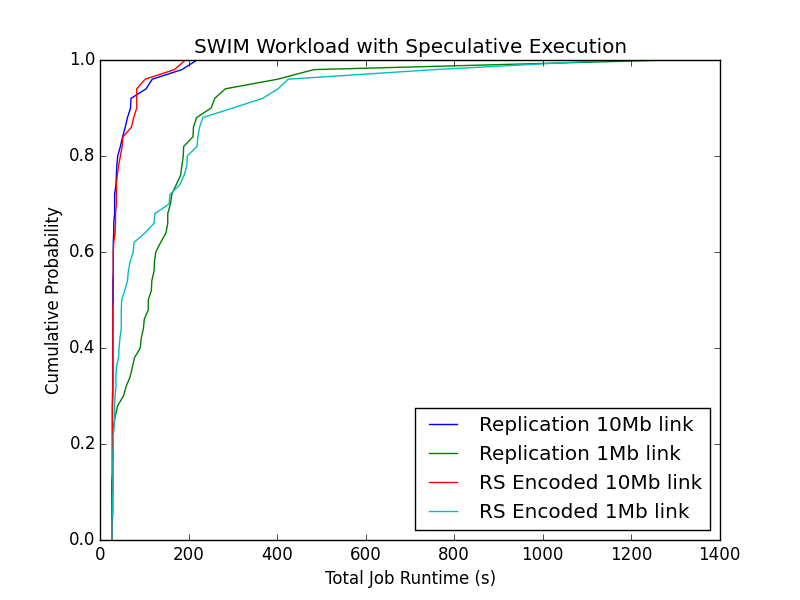
\includegraphics[scale=0.6]{plots/swim.png}
        \caption[SWIM Workload Test]{Running SWIM workload shows no decreased
            performance when using erasure encoded storage and speculative
        execution}
        \label{swim}
    \end{figure}

    The SWIM workload simulates the workload found on Facebook's Hadoop
    clusters. It is expected that the job runtime when using erasure encoded
    storage and speculative execution is longer than that of jobs using
    replication and speculative execution. What we see in \ref{swim} is that
    this is not the case and both storage methods seems to perform equally. This
    is the result of the SWIM jobs operating on input data that is small and
    requires only a few maps tasks. Because of the small number of map tasks,
    speculative attempts are never actually made. This means that regardless of
    the storage method, a task assigned to read a block over a slow network link
    will finish reading from that block without being preempted by a faster task
    or slowed down by a backup task reading over the same link. In order to get
    results that show how speculative execution affects performance when using
    replication and erasure codes, larger input data sets must be used that
    require enough maps tasks for speculative tasks to be launched.

    \section{Problems with HDFS-Raid}

    HDFS-Raid \cite{HDFS-Raid} provides a block placement policy called
    \code{BlockPlacementPolicyRaid} which tries to avoid co-located stripe
    blocks by placing each stripe block on a distinct datanode. I was unable to
    get this working due to incompatibilities between HDFS-Raid 0.22.0 and
    Hadoop 0.23.11. Instead, the default placement policy was used and a node
    containing only one file block was chosen to have its network slowed during
    testing.

\end{appendices}

%------------------------------------------------------------------------------%

% Format a LaTeX bibliography
\bibliographystyle{plain}
\bibliography{bibliography.bib}{}

% Figures and tables, if you decide to leave them to the end
%\input{figure}
%\input{table}

\end{document}


